\chapter{Implementation}\label{chap:implementation}

%\textbf{the  writing plan:}
%\begin{itemize}
%\item Introducing Java FX Description pane
%	\begin{itemize}
% 	\item besonderheit für build (maven anpassungen)
%		\item Problem JavaFX auto beenden
%	\end{itemize}	
%\item explain exactly how the cids renderer are selected and displayed.
%\item first idea, Description Pane distinguish the usage of web renderer
%\item better approach to implement the "coc changes" in the renderer factory
%\item Designing an interface for the communication 
%		\begin{itemize}
%			\item bridge object
%			\item update problematic, bulk update for cidsBean
%	\end{itemize}
%\item Testing and Problems
%		\begin{itemize}
%			\item long time for initialisation
%			\item problem style of combobox elements
%		\end{itemize}
%\item Development of an Angular based example renderer for Vermessungrisse
%\end{itemize}

\section{Integrating the JavaFX WebView}

\subsection{JavaFX WebView based DescriptionPane}

As a first step it is necessary to integrate the JavaFX WebView into the description pane of the navigator.
As already mentioned the description pane already supports the visualisation of HTML pages to offer additional information for the selected catalogue object. 
Hence the JavaFX WebView offers much more features than the already used browser APIs (cf \ref{chap:browser_api_comparison}), a useful benefit can be reached using the WebView as browser API also for that case. 
To ensure a full backward compatibility the usage of the JavaFX WebView is implemented in a configurable manner. 
The description pane is mainly implemented as an abstract class \texttt{DescriptionPane}. 
This class represents a \texttt{JPanel} and offer basic functionality like the distinction when to load a HTML page or a cids renderer and the loading mechanism for cids renderer. 
Using a abstract class easily allows to extend the functionality of the \texttt{DescriptionPane} that uses different browser API's.  
Figure \ref{fig:class_diag_desc_pane} depicts a class diagram of the \texttt{DescriptionPane} and related classes.

\begin{figure}
	\centering	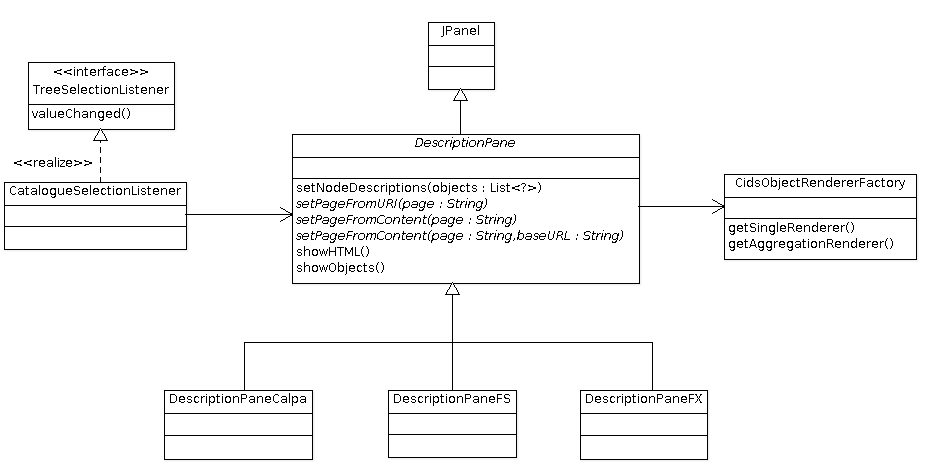
\includegraphics[width=1.0\textwidth]{./img/classDiagramms/description_pane.png}
	\caption{DescriptionPane and relating classes}
	\label{fig:class_diag_desc_pane}
\end{figure}

The \texttt{DescriptionPane} panel uses a \texttt{CardLayout} to separate the visualisation of cids renderer from the visualisation of HTML pages.
The \texttt{CardLayout} easily allows to programmatically switch between multiple and different panels based on unique names, without taking care of refreshing the GUI by hand.
Using this approach the implementation classes of the \texttt{DescriptionPane} can easily implement their own logic and define the tools they use to visualise HTML description pages.
It is just necessary to add a panel to the \texttt{DescriptionPane} with the correct identifier that is used in the abstract class.
The three abstract methods shown in figure \ref{fig:class_diag_desc_pane}, are used to provide the HTML encoded information that shall be displayed.

Which concrete implementation of the \texttt{DescriptionPane} is used, is determined during the navigator start and depends on the configuration made in the navigators configuration file.
During the navigator start, the \texttt{PropertyManager} class loads the configuration file of the navigator and caches the settings.
For each property the \texttt{PropertyManager} has corresponding getter and setter functions.
It is implemented as a singleton, which easily allows to use it everywhere where access to the settings is needed.
There are already two existing implementations that uses different browser APIs.
Hence the current implementation uses Calpa API as default case, there is only one boolean property called \texttt{useFlyingSaucer} that indicates to use the \texttt{DescriptionPaneFS} class, a description pane that uses the  FlyingSaucer API.
One possible solution for introducing a JavaFX based description pane is to introduce a new property similar to the already existing one.
Following this approach has the drawback that there are different properties for configuring the same functionality.
Furthermore, the name of the \enquote{\texttt{useFlyingSaucer}} property does not indicate very well what functionality is exactly configured.
Therefore a new text property \enquote{\texttt{navigator.descriptionPane.htmlRenderer}} is introduced, whose value determines which concrete implementation of the \texttt{DescriptionPane} shall be used.
To ensure backward compatibility the old properties are still supported, but when they are used a warning is written to the logging mechanism of the application.
Additionally, the \texttt{DescriptionPaneCalpa} still functions as fall-back case if no or a invalid value for the property is configured.

For the JavaFX WebView based description pane, a new class \texttt{DescriptionPaneFX} is generated, that uses a \texttt{JFXPanel} that contains a Java FX WebView for visualising HTML content.
This panel is then used within the \texttt{CardLayout} of the description pane as described above.
The \texttt{JFXPanel} is a Swing component that acts as JavaFX application runtime container and eases the integration of JavaFX components into Swing.
Normally when developing JavaFX applications, it is necessary to extend the JavaFX \texttt{Application} class, which initializes the JavaFX runtime environment and automatically calls a \texttt{start(Stage primaryStage)} method that needs to be implemented when extending the \texttt{Application} class.
Important to note is the parameter of this method.
A stage object is a top level GUI container that can have several scenes.
The scenes itself are also container classes for contents.
This architecture is based on the principal idea of a theatre play.
The stage on a theatre contains multiple scenes, each with a custom look and behaviour.
The stage object is already constructed by the \texttt{Application} class and it is just necessary to set a scene object on that stage.
When using a \texttt{JFXPanel}, there is no start method that can be executed.
Therefore the \texttt{JFXPanel} initializes the JavaFX runtime environment during construction time.
The only thing what needs to be done is to set a scene that should be visualised by the \texttt{JFXPanel} which in our case is the WebView.
Figure \ref{fig:class_diag_desc_pane_fx} demonstrates the class structure of the FX based description pane.

\begin{figure}
	\centering	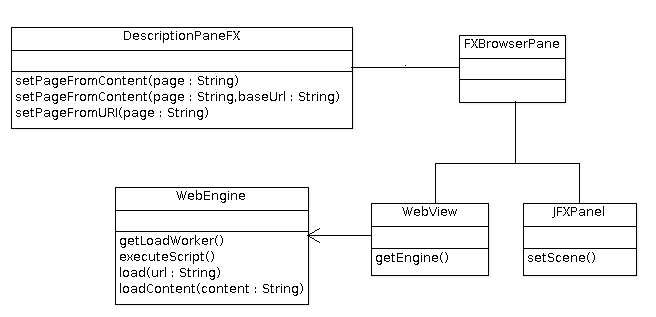
\includegraphics[width=1.0\textwidth]{./img/classDiagramms/desc_pane_fx.png}
	\caption{DescriptionPaneFX and relating classes}
	\label{fig:class_diag_desc_pane_fx}
\end{figure}

Using JavaFX dependent classes requires to integrate the JavaFX library into the classpath.
Although this library is shipped with the JRE since Java SE 7 update 6 (7u6), it is not part of the default classpath that is used when building and starting Netbeans projects. Thus, it is not possible to use and built programs that use JavaFX dependent classes within the Netbeans IDE.
Possible solutions to this issue are discussed in \autocite{impl:fx-classpath}.
The first approach is to move the corresponding jar file into a folder that is on the classpath by default, like the ext-folder of the JRE.
This has the disadvantage that this adoption needs to be done on every client.
Therefore an other solution is preferred.
The jfxrt.jar gets defined as system dependency.
System dependencies are always available and are not looked up in the maven specific repository, hence maven assumes that these dependencies are explicitly provided.
Thus way, the JavaFX dependency can be defined in a system and JRE independent way.
Additionally it is necessary to add the library to the classpath that is created from Maven for running the application and to avoid a \texttt{java.lang.NoClassDefFoundError} when running the application.
 
During the development, two problems occurred.
The first one was an \texttt{Illegal} \texttt{StateException: Not on FX application thread} Exception.
The reason for this is quite simple and is based on the fact, that JavaFX components can not be accessed outside the JavaFX application thread.
This is similar to JavaSwing where Swing components should also be accessed only from the Event Dispatch Thread, with the difference that violating this constraint leads to an exception when trying the same in JavaFX.
This was a conscious decision from the JavaFX developers hence accessing Swing components outside the Event Dispatch Thread is one of the most reason for errors.

The second problem occurred, when switching between a object node that nudges the description pane to load and show a Swing based cids renderer and a node with an HTML description page.
When switching back to the HTML description again an \texttt{IllegalStateException} is thrown, with the message \texttt{\enquote{Platform exit has been called}}.
The reason for this is the implementation of the \texttt{JFXPanel}.
Hence the \texttt{JFXPanel} automatically starts the JavaFX runtime environment, it must also ensure it is terminated when it is no longer necessary.
This is the case when the scene object that the \texttt{JFXPanel} displays is finished and the panel is no longer visible.
Hence we use the \texttt{JFXPanel}in a \texttt{CardLayout} the \texttt{JFXPanel} implicitly calls the exit method of the JavaFX platform which terminates the JavaFX environment.
This implicit termination can be suppressed by setting a parameter with the following code:

\begin{lstlisting}[label=implicit_exit,caption=Disable JavaFX implicit exit]
Platform.setImplicitExit(false);
\end{lstlisting}

\subsection{Adopting the Convention over Configuration Mechanism}

Up to this point the JavaFX WebView is already integrated into the navigator, but it is still not possible to visualize html applications as renderer for object nodes.
As mentioned above, the abstract class \texttt{DescriptionPane} is responsible for loading the corresponding renderer for object nodes.
To fully understand what possibilities exists to implement the pending feature, it is necessary to have a closer look on that mechanism.
When selecting a node in the cids catalogue, the \texttt{CatalogueSelectionListener} gets notified about this.
The \texttt{CatalogueSelectionListener} calls the \texttt{setNodeDescription} method on the \texttt{DescriptionPane}
This method makes a series of decisions what exactly should be displayed.
 
The first idea to show HTML applications as cids renderer is to customize this method and implement the necessary changes there.
Since there can be different description pane implementations, but only the \texttt{DescriptionPaneFX} can display complex web applications it is necessary to overwrite this method there.
The code needs to be changed to implement the following logic.
If the selected node is a object node, it is necessary to check if for the corresponding cids class the new introduced class attribute \texttt{isHtmlRenderer} is configured.
If so, the value of the class attribute  points to the location of the web application.
This URL can be used to call the \texttt{setPageFromURL()} method of the \texttt{DescriptionPaneFX}.
%Furthermore the panel that contains the JavaFX WebView needs to be displayed.
%Listing depicts the new behaviour in pseudo-code

%\todo{add listing in pseudo code}

The drawback of this approach is, that it will only work when the new JavaFX based description pane is used and will not work with the other description pane implementations.
Furthermore this approach will not fit perfectly into the conceptual design that strictly separates the display of renderer components and description pages.
Therefore a more appropriate solution is to adopt the factories that are responsible for loading the cids renderer and editors for a cids class.
As figure \ref{fig:class_diag_desc_pane} depicts the \texttt{CidsObjectRendererFactory} has two different methods for retrieving single and aggregation renderer.
The cids system also allows the definition of so called aggregation renderer which can visualise aggregated information of multiple objects of the same class.
If no aggregation renderer is defined, or objects of different classes are selected, the single renderer for each object are vertically stacked in the description pane.
Therefore it is just necessary to adopt the \texttt{getSingleRenderer} method with the above mentioned changes.

The \texttt{CidsObjectRendererFactory} needs to return a \texttt{JComponent} that represents the cids renderer.
Hence the only difference for web renderer components is the URL that  points to the location of the web renderer which is configured in the isHtmlRenderer class attribute, it is easily possible to develop a new renderer class \texttt{HTMLWidgetRenderer} that uses also a \texttt{FXBrowserPanel}, and is parametrisable  with the URL of the web application.

In fact this component can also be used for visualising web based editors, class inheritance can be used to inherit the needed functionality from the editor to the renderer and allows the same code base for both cases.
However, this approach heavily relies on the assumption that renderer and editors for single objects have only a different intentional usage and no different graphical user interfaces .
A renderer visualizes information whether a editor can be used to edit the data.
Using the same code base for editors and renderer is a very common practice that is  already used in many cases when developing cids renderer and editors.
Using the same GUI for editors and renderer is possible when all input fields of the editor are disabled.
Thus, this needs to be regarded when developing web renderer components.
Regarding this, the class structure depicted in figure  \ref{fig:class_diag_html_widget_editor} is implemented.

\begin{figure}
	\centering	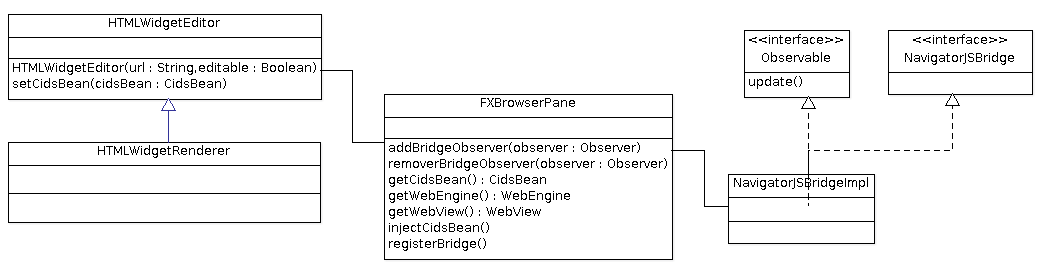
\includegraphics[width=1.0\textwidth]{./img/classDiagramms/html_editor.png}
	\caption{HTMLWidgetEditor and related classes}
	\label{fig:class_diag_html_widget_editor}
\end{figure}

Important to note, is the \texttt{editable} parameter in the constructor of the \texttt{HTMLWidgetEditor}.
This parameter can act as a flag if  the web renderer component shall be used in editor or renderer mode, which means that input fields are disabled to avoid data changes.
As figure \ref{fig:class_diag_html_widget_editor} depicts, the \texttt{HTMLWidgetEditor} implements the \texttt{setCidsBean} method, which is called when the renderers and editors are loaded, to inject the object into the renderer.
To enable the usage of web applications as cids editors, the only thing left to do is to adopt the \texttt{CidsObjectEditorFactory} in the same manner as the \texttt{CidsObjectRendererFactory}.

\section{Development of an Angular based renderer}

In a next step a web renderer and editor component is implemented, that facilitates testing the implemented state.
Therefore it is necessary to implement an Angular based demo application that can be integrated in the cids navigator as renderer and editor.
Without such an application it would be difficult, if not impossible, to test above mentioned enhancements.

For developing a demo application, an already existing render and editor with a complex cids data model shall be used and re-implemented in a web application with the same functionality .
In WuNDa, an information system based on cids and the cids navigator, it is possible to manage survey plans.
The survey plans are a good candidate for a demo application hence their underlying data structure contains every possible data relation that can be modelled with cids.
Figure \ref{fig:survey_plan_data_model} depicts the cids data structure of the survey plans.
This data structure is also reflected by the \texttt{CidsBean} that need to be injected into the renderer components.
The \texttt{CidsBean} acts as the main model for the Angular application.

\begin{figure}
	\centering	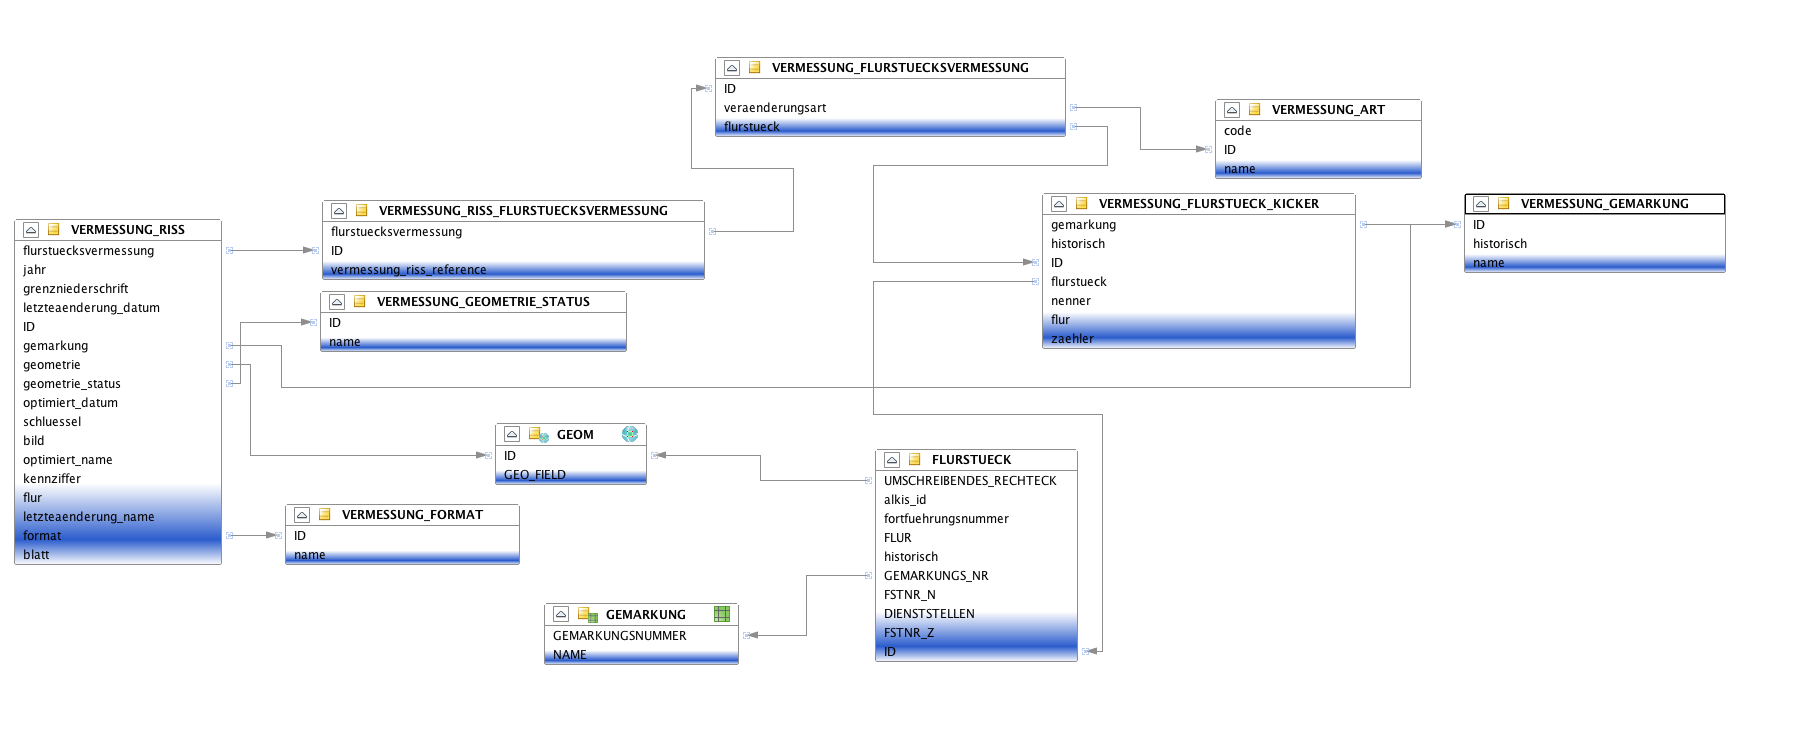
\includegraphics[width=1.0\textwidth]{./img/impl/surveyPlan_data_model.png}
	\caption{Cids data model of survey plans}
	\label{fig:survey_plan_data_model}
\end{figure}

Before starting with the implementation of the Angular based web renderer, the functionality of the already Swing based implementation of the survey plan renderer and editor is explained.
Figure \ref{fig:survey_plan_swing_editor} shows the Swing based implementation of the survey plan editor.
Besides visualising the main information relating to a survey plan (part a in figure \ref{fig:survey_plan_swing_editor}),  it is also possible to edit the land parcels that are affected of the survey plan (part b in figure \ref{fig:survey_plan_swing_editor}).
Area c in figure \ref{fig:survey_plan_swing_editor} shows that the survey plan renderer can also visualise images of historic survey plans documents.
Thereby, zooming and panning the image is possible.
The renderer basically has the same functionality, with the exception that not all information are visualised and it is not possible to change any data.
Because implementing the visualisation of historic survey plan documents is more difficult and not mandatory for using and testing the application, this feature is excluded in a first step and can be added later on.

\begin{figure}
	\centering	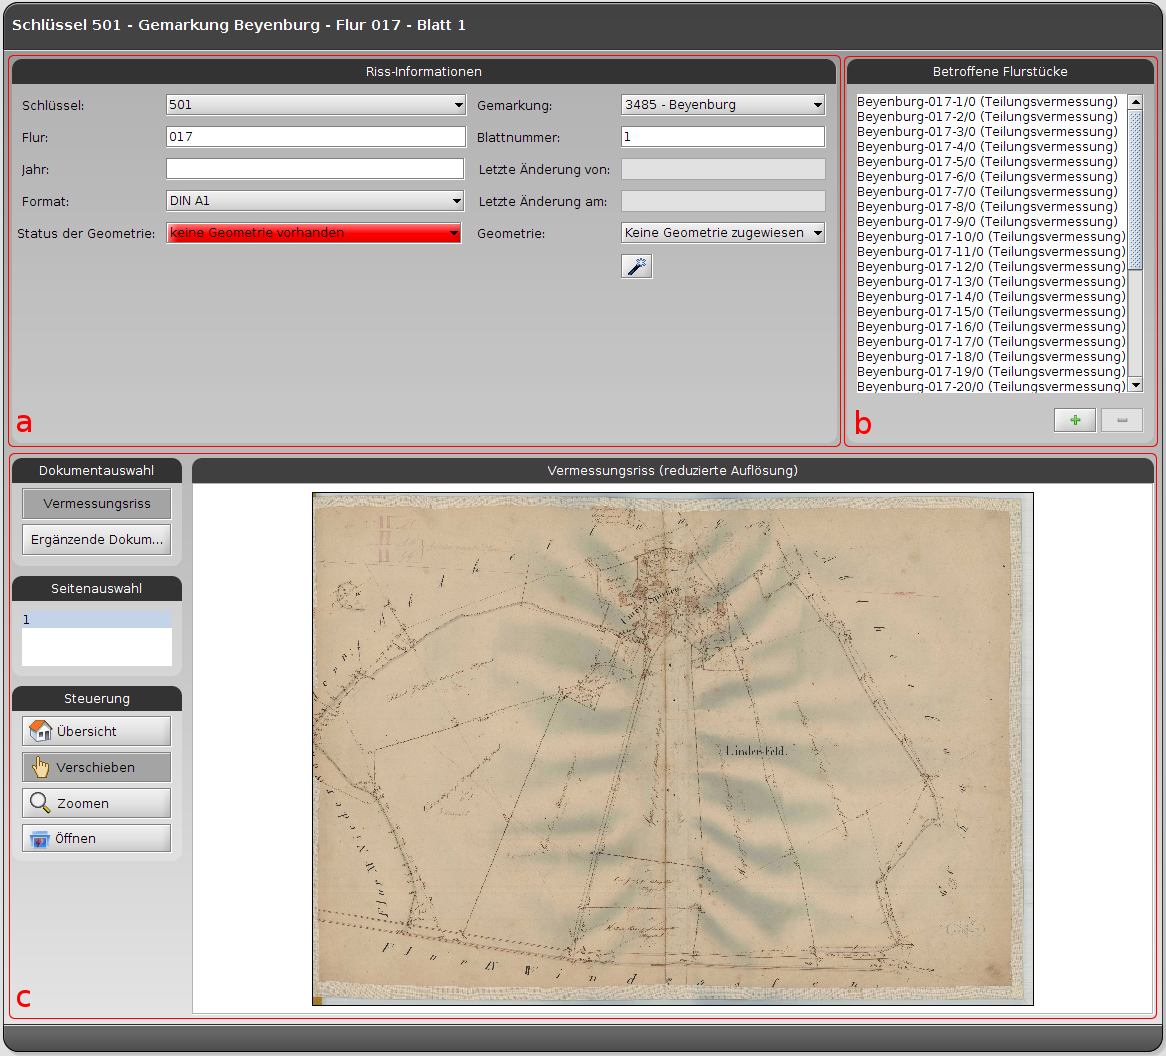
\includegraphics[width=1.0\textwidth]{./img/impl/survey_plan_editor_old.png}
	\caption{Swing based cids editor for survey plans}
	\label{fig:survey_plan_swing_editor}
\end{figure}

In fact no data exchange between the navigator and the web application is currently possible, it is required to load the data of an example object from a file until the data exchange between navigator and web applications is implemented.
According to the usual practice when developing web applications, the data is represented in the JSON format.
Hence the objects in the navigator are usually represented as Java \texttt{CidsBean} objects, it is necessary to transform and extract the data of a survey plan object into the JSON format.
For this the \texttt{CidsBean} class offers a set of helper methods that can be used.  



\lstinputlisting[label=lst:demo-ng-app-1,caption=HTML markup of the demo application]{./listings/impl/demo_app/index.html}
\lstinputlisting[label=lst:demo-ng-app-2,caption=Controller function of the demo application ]{./listings/impl/demo_app/app.js}


A first implementation of the Angular based renderer has a very simple structure.
Listing \ref{lst:demo-ng-app-1} and \ref{lst:demo-ng-app-2} represents the important parts of the implementation.
For the whole application, one controller with one scope can be used.
The controller is defined with the built in directive ng-controller.
This directive points Angular, to use the \texttt{SurveyPlanController} function as the controller function for the application.
The controller loads the JSON formatted representation of the survey plan generated in the previous step.
For this, Angular already offers the \texttt{\$http} service which eases the retrieval of resources in an asynchronous way.
When the JSON object is completely loaded, the object can be attached to the \texttt{\$scope} of the controller.
In the view we can easily bind properties of the object to arbitrary elements within the view.
The look of the application can be easily adopted with some additional style sheets to gain a similar design to the already existing swing components. This supports a seamless integration into the cids navigator.
Figure \ref{fig:survey_plan_angular_editor} shows a screenshot of the styled application.

\begin{figure}
	\centering	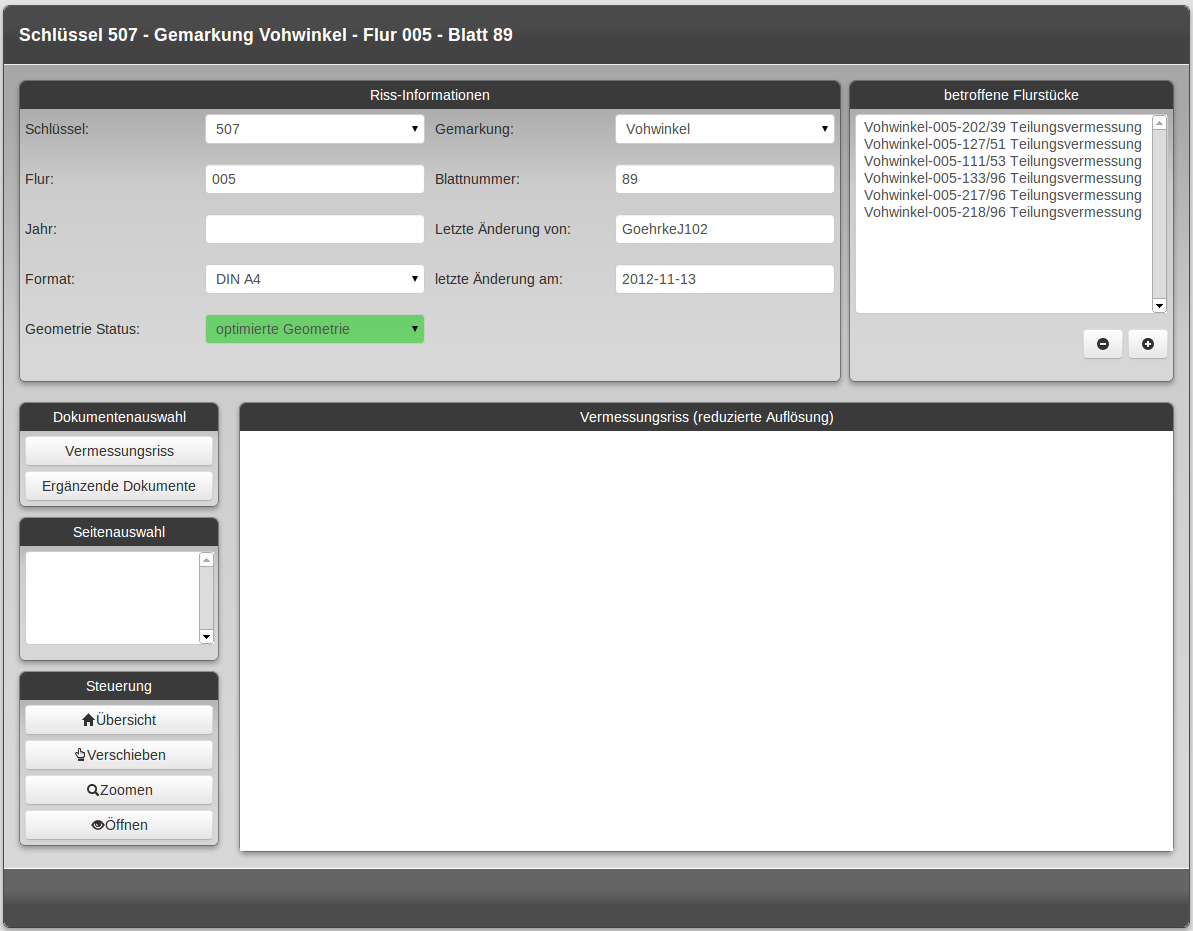
\includegraphics[width=1.0\textwidth]{./img/impl/survey_plan_editor_new_alpha.png}
	\caption{Angular based cids editor for survey plans}
	\label{fig:survey_plan_angular_editor}
\end{figure}
 
There are still some remaining issues that distinct the web application from the Swing based one.
As already mentioned, the same application shall be used as renderer and editor.
This means in the case of the demo application that it is necessary to disable the input elements as well as hiding some data fields that are not necessary when the application shall be used as renderer.
Therefore a new property called \texttt{isRenderer} is added to the scope, that indicates if the application shall be used in renderer or editor mode.
This property can be used to hide parts of the view and to change the styling of the input fields.
Again, Angular is prepared with built in directives that allow an easy implementation of both features.
The ng-hide directive hides arbitrary HTML elements based on the expression that is provided to it.
For disabling the input fields, the \texttt{ng-disabled} directive can be used.
To both directives it is sufficient to bind the \texttt{isRenderer} property to them.
When integrating the demo application into the navigator it is necessary to correctly set the \texttt{isRenderer} property depending on the usage as renderer or editor.
This is described extensively in the next chapter.

Another important difference between the Angular and the Swing based application is how 1-n relations of the data model are visualised to the user.
An example is the format field of the survey plan document. A survey plan has a format and there is a fix set of formats that exists. 
In the Swing application \texttt{ComboBoxes} are used to offer the user this fix set of elements of the related cids class..
The \texttt{CidsBean} that represents a survey plan only contains just the currently selected element of the related cids class however.
In the Swing based application the missing elements are loaded in the background.
A same approach needs to be implemented in the Angular based application but requires a working data exchange between the navigator and the web application which is still pending.
To ease the integration of this feature afterwards, a Java Script function that loads all elements of a given cids object is implemented.
Hence no data exchange with the cids system is possible, those information are also loaded from a json file based on a naming convention.
The following examples demonstrates this.
For the format example above this method tries to load a file \texttt{format.json} from the server.
This data can then be used to create select elements that offer all existing format objects.
Hence such a select element is a very common and frequently used feature, it is appropriate to implement it as a reusable component.
This can be reached with an Angular directive.

The features, adding land parcels to the survey plan, setting a geometry that represents the survey plan and visualising historic survey plan images, all require a working data exchange between the navigator and the web application, or are not essential for using the web application as renderer, or editor respectively, in the navigator. 
Thus in the next step, the data exchange between the navigator and web applications is implemented first.

\section{Establishing bi-directional data Exchange}

%The HTMLWidgetEditor class implements the CidsObjectRenderer interface which forces the HTMLWidgetEditor class to implement the setCidsBean method. Those method is called from Navigator to inject the data into the renderer.   

With the current state it is already possible to visualise HTML applications as object renderer and editors within the navigator, but what is still missing, is the data exchange between the navigator and the web applications.
 
As outlined in chapter \ref{chap:browser_api_comparison}, the JavaFX WebView allows a bi-directional communication between the loaded web page and Java.
For the first direction, the communication from Java to the web application, the JavaFX WebEngine has a method \texttt{executeScript()}, which allows the execution of arbitrary JavaScript code in the  context of the currently loaded page.
Furthermore, the WebEngine gives full access to the Document Model (DOM).
The DOM can be accessed using Java DOM core classes and allows the manipulation of the DOM programmatically.
 
Hence Java and JavaScript have a totally different type system, there needs to be a type conversion when exchanging data between Java and JavaScript.
In \autocite{impl:java2js-data-conversion}  a very detailed explanation of the conversion rules is given.
Hence this conversion for simple types is rather obvious, the important part to mention is that JavaScript objects, which can not be easily transferred into simple Java types, are wrapped as an instance of the \texttt{JSObject} class.
The same conversion is used if the result of the executed JavaScript code is a DOM node.

For making upcalls from JavaScript to Java the concept is to create and register a bridge object, which can be an arbitrary Java object.
This bridge object must be accessible in the JavaScript context. 
This can be reached by calling the \texttt{setMember} method on a \texttt{JSObject} object.
Subsequent, it is possible to access any public fields and methods of the Java bridge object in the JavaScript context.
Since the bridge object is registered to a \texttt{JSObject}, it is possible to attach the bridge object to any JavaScript object or DOM node.
Again a type conversion, that behaves in the inverse way when converting from JavaScript to Java types is applied.

In fact the bridge object can be registered at an arbitrary DOM node or JavaScript object, it is necessary to establish a common interface on which the bridge object always is registered to allow a unified usage within the web application context.
Furthermore this interface needs to offer the possibility to inject data.
This is necessary in fact the selected catalogue object also gets injected from the navigator into the editor.
Just if this happens, it is possible to forward this data to the web application.

Since it is necessary to regard the usage of the web renderer component also without the navigator this  behaviour needs to be abstracted from the application itself.
This is reached by separating the web renderer component from the context it is executed in, with an additional layer.
Figure \ref{fig:cidsJS} gives an overview of the architectural design.

\begin{figure}
	\centering	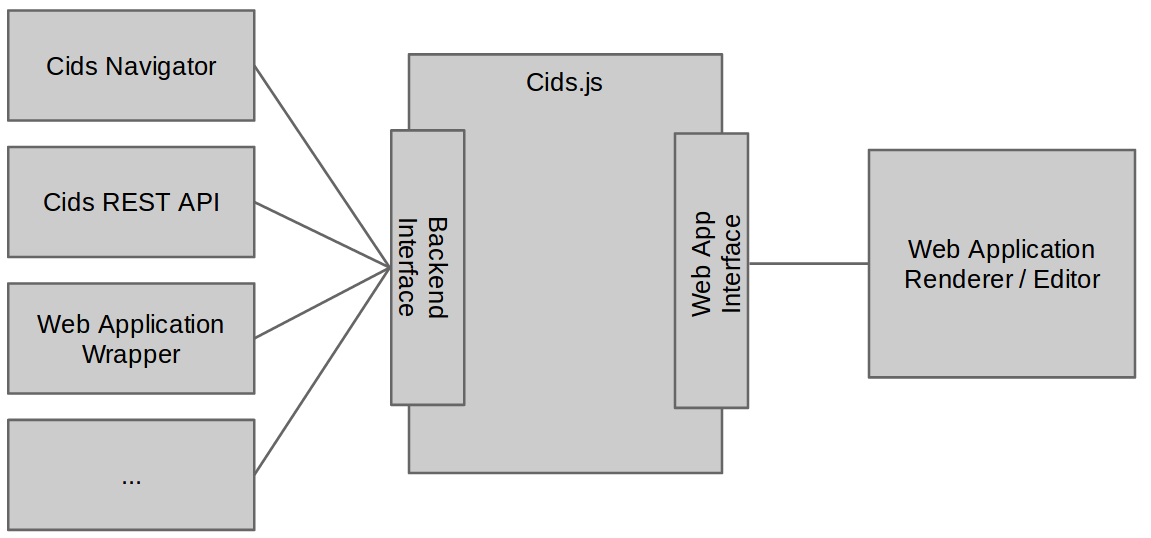
\includegraphics[width=1.0\textwidth]{./img/impl/cidsJS.png}
	\caption{Architectural Overview CidsJS}
	\label{fig:cidsJS}
\end{figure}

The web renderer component shall only communicate with the cidsJS layer which abstracts the context the web renderer component is executed in.
As depicted in figure \ref{fig:cidsJS} the cidsJS layer needs to define fix interfaces for both sides, the client side, and the backend side, hence especially the navigator needs to inject data into the application context and needs to register a bridge object for data exchange.
The cidsJS layer is represented as a JavaScript object that can be easily accessed within the whole JavaScript context of the loaded page and thereby is easily accessible within the Java scope.
A very common practice for this is to use an anonymous function that handles the initialisation of the cidsJS layer object and finally exposes this object to the global scope of the application afterwards. 
A similar approach is used in other frameworks such as JQuery or Prototype.
Placing the initialisation function in a separate file it is sufficient to include this file with a script tag in the index file of the application to use the cidsJS layer object.
Owing to the exposion of the cidsJS object to the global JavaScript scope, it is very easy to get a reference of the cidsJS object in Java as listing \ref{lst:inject_bean} demonstrates.
 

\begin{lstlisting}[label=lst:inject_bean,caption=Injecting the cidsBean to the JavaScript application]
JSObject cidsJs = (JSObject)webEng.executeScript("ci");

 cidsJs.call("injectCidsBean",
              CidsBean.getCidsBeanObjectMapper().writeValueAsString(bean));
\end{lstlisting}
%Seperating the communication of the web application and the navigator with an additional layer hides the context the application hosted in, for example the cids Navigator, from the application itself and eases the usage in other contexts. Therefore cidsJS, allows the usage of several backend implementations and forwards the requests of the web application to the currently used backend.The second important part of the cidsJS layer is responsible to define a fix place where the bridge object that allows the communication between Java and JavaScript can be registered and offers an interface that allows to inject vital data to the web application, like the cidsBean and if the application acts as editor or renderer.

The first thing that is implemented is the injection of the cidsBean which represents the selected catalogue object.
For this cidsJS is extended with a respective method called \texttt{injectCidsBean}.
When the setCidsBean method of the \texttt{HtmlWidgetEditor} is called, the \texttt{injectCidsBean} method can be used to provide the web application context with the necessary data.
Sequence diagram  \ref{fig:seq-diag-data-exchange-1} demonstrates the single steps that are executed to injected the  \texttt{CidsBean} into the web application.
The same approach can be used for setting the \texttt{isRenderer} property that indicates if the application shall be used in render or editor mode.

Injecting the cidsBean into the JavaScript context is only a part of the solution.
The \texttt{SurveyPlanController} must also be adopted to the new situation.
Therefore cidsJS is extended with a method \texttt{getCidsBean} that is called from the \texttt{SurveyPlanController} during the initialisation.
Hence there is no guaranteed order that the\texttt{SurveyPlanController} is initialised after the \texttt{CidsBean} was injected into cidsJS, the initialisation of the controller needs to be delayed.
Therefore the \texttt{getCidsBean} method returns a promise object.
Promises are a very common concept in JavaScript to handle asynchronous events.
A promise is an object that represents the result of an action that is performed asynchronously and may or may not finish at any given point in time.
Angular already provides a promise implementation that allows to register so called callback-functions for different cases.
Different callback-functions can be registered for the case the result is available or a failure has happened.
The \texttt{\$http} service, that was used to load relevant data from file so far, also uses Angular’s promise implementation.
Angular uses a so called defer object, that can be used to programmatically reject or resolve a promise which will execute the registered callback functions for the respective case.
In our case this defer object is initialized during the initialisation of cidsJS and resolved when the injectCidsBean method is called. The sequence diagramm \ref{fig:seq-diag-data-exchange-1} demonstrates the steps that are executed during the initialisation process.

\begin{figure}
	\centering	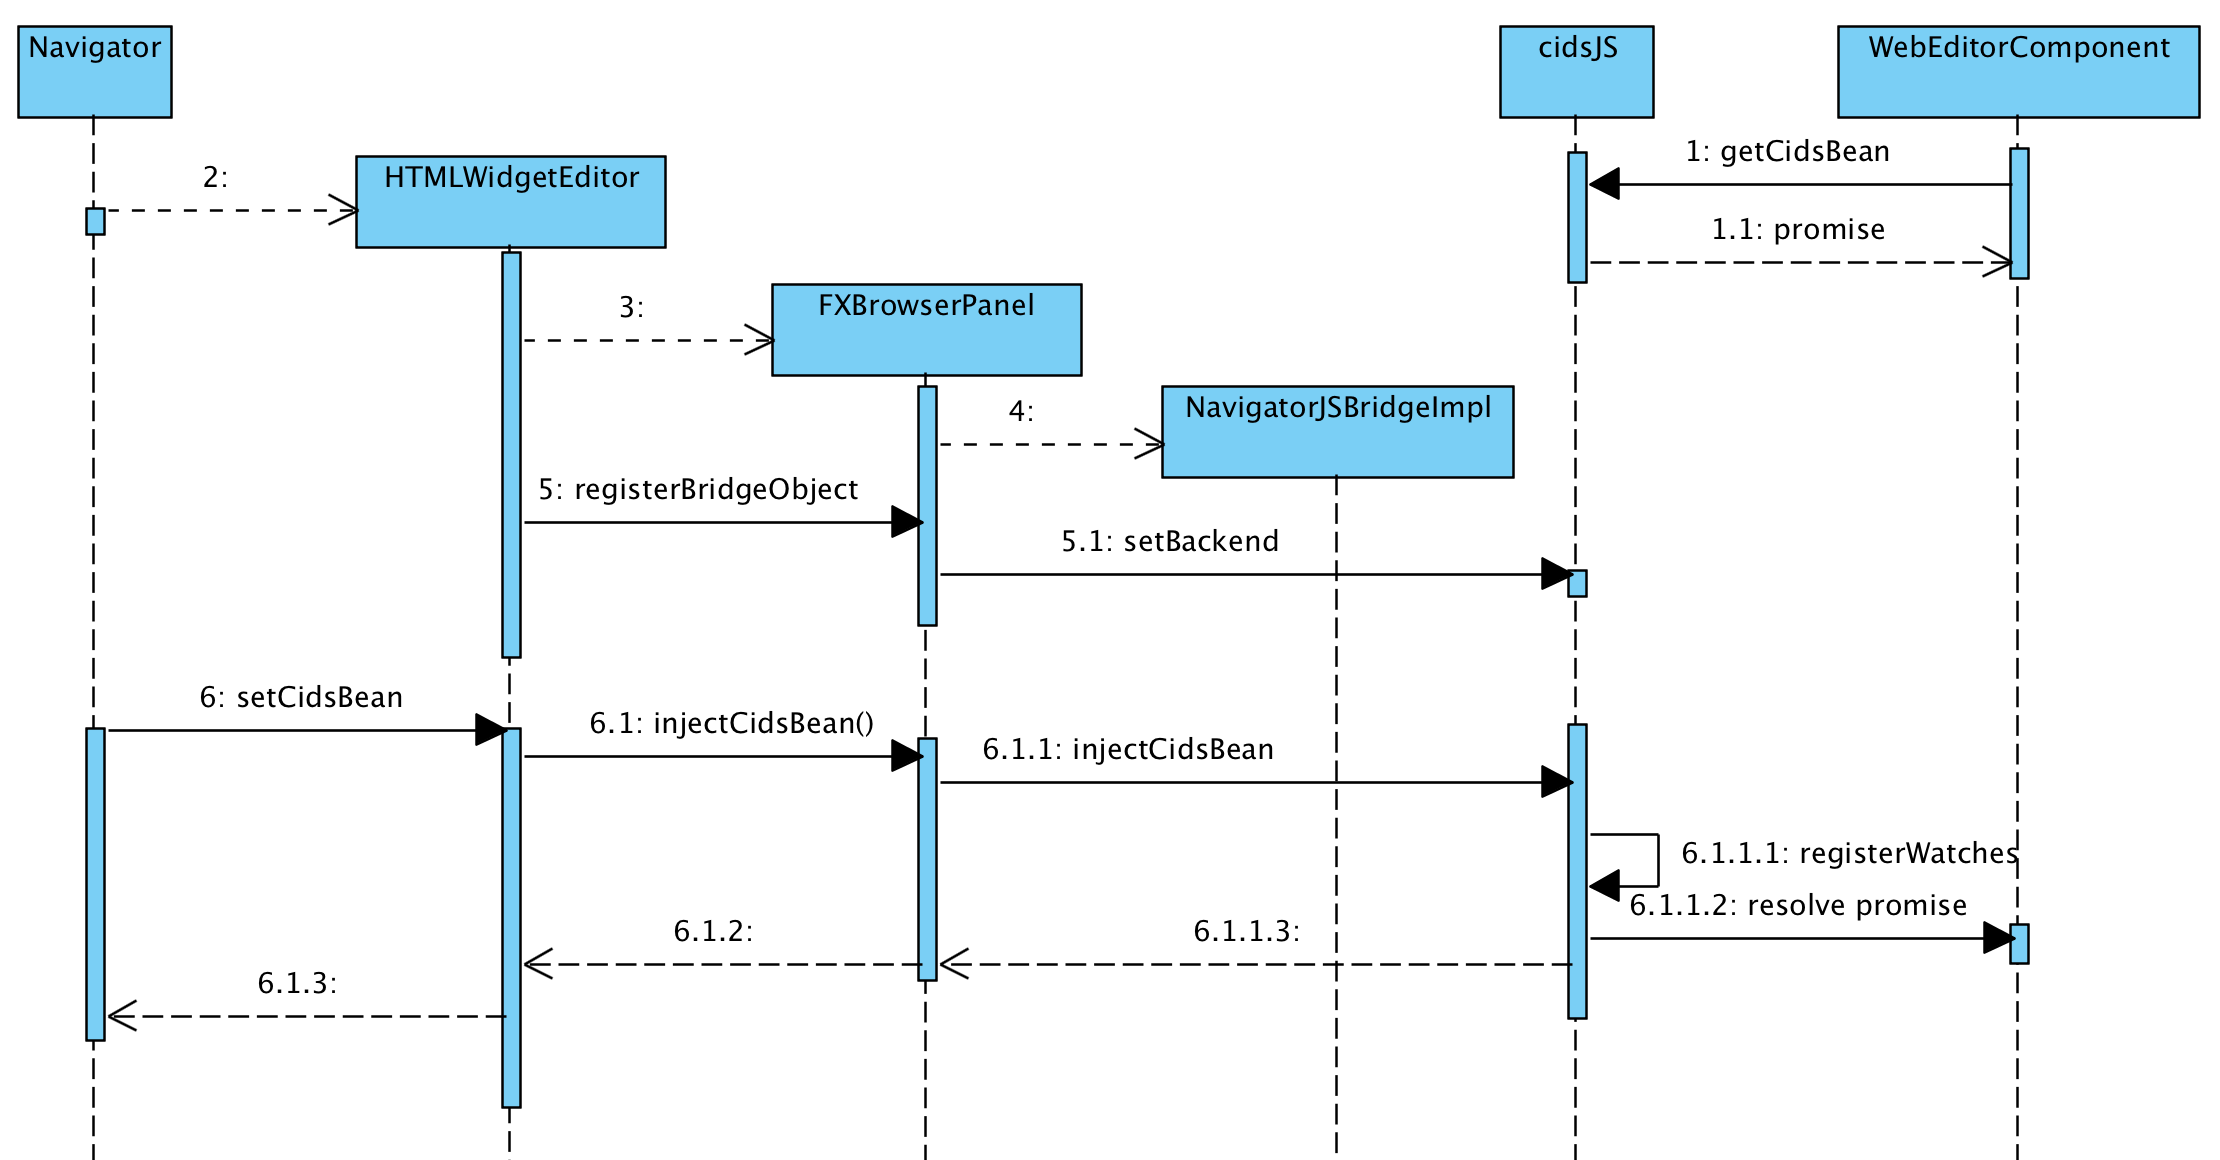
\includegraphics[width=1.0\textwidth]{./img/classDiagramms/seq_diag_data_exchange.png}
	\caption{Injecting cidsBean into the web renderer component}
	\label{fig:seq-diag-data-exchange-1}
\end{figure}

Figure \ref{fig:nav_web_renderer} shows the usage of the developed web renderer component within the navigator.
However, using the demo application as editor is still not possible in fact only a one way data exchange is implemented so far. 
Changing the data in the web editor component is out of the scope of the cids navigator. 
The following section describe how the data exchange from the web editor component back to the cids navigator is implemented.

\begin{figure}
	\centering	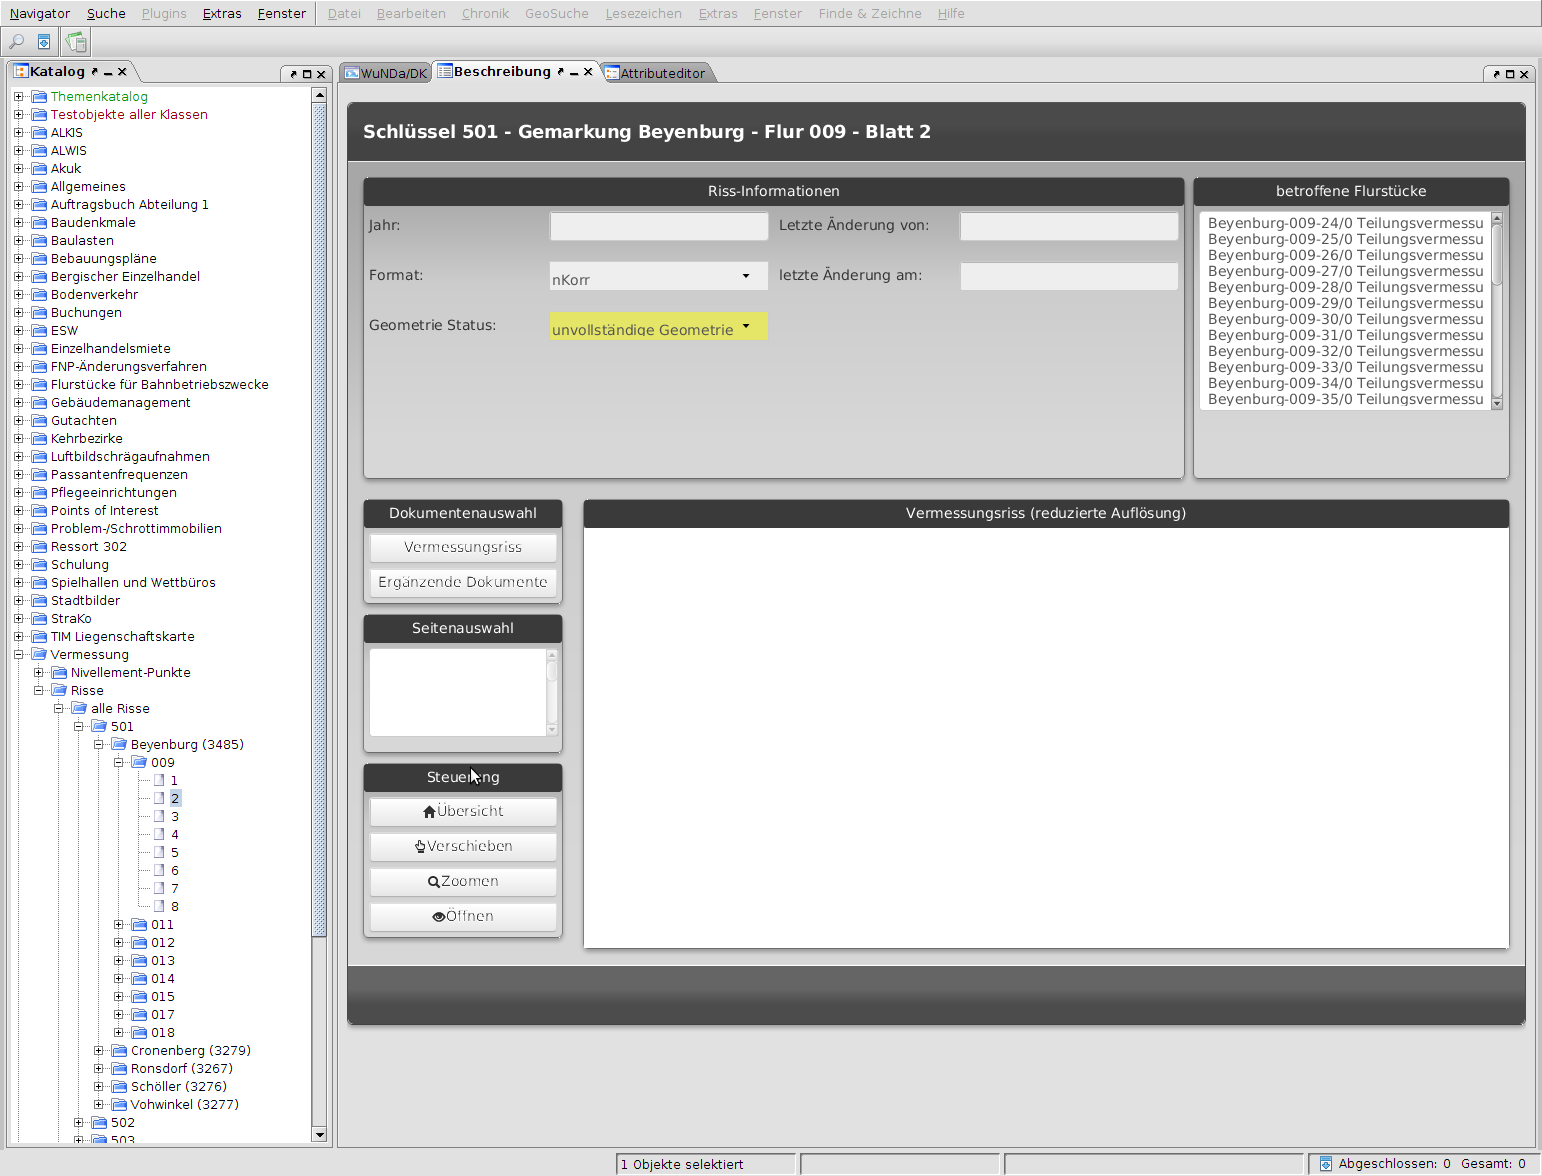
\includegraphics[width=1.0\textwidth]{./img/impl/navigator_web_renderer.png}
	\caption{Navigator with Survey Plan Web Renderer}
	\label{fig:nav_web_renderer}
\end{figure}

The panel in that editors are embedded in the navigator offers buttons for saving and discarding changes that are made to the \texttt{CidsBean} object.
If it was not changed, the editor is closed.
In the case the object has changed, a dialog that calls on the user to confirm the action is shown.
The \texttt{CidsBean} itself provides two different flags, that indicate if the \texttt{CidsBean} was changed.
The first one, is set automatically if a value of a property has changed.
The \texttt{CidsBean} therefore implements a \texttt{PropertyChangeListener} which allows to listen on every property change.
The second flag can be used to artificially mark the \texttt{CidsBean} as changed.
The problem when using a web editor component, is that the save and discard actions are initiated by the user and within the context of the navigator.
At this point the information if the \texttt{CidsBean} has changed needs to be already available.
Therefore, simply setting the artificial change flag in the \texttt{HTMLWIdgetEditor} is not sufficient, in fact this marks the bean always as changed and modifies the behaviour of the save and discard button described above.
 
In contrast to the first approach the only possible way to ensure the same application logic, is to notify the navigator about every change of the \texttt{CidsBean} that happened in the web editor context.
Hence this is only necessary when the application is used within the navigator, the cidsJS layer is extended with the respective functionality.
When the \texttt{injectCidsBean} method in cidsJS is called, cidsJS registers Angular watches on every property of the cidsBean object.
An Angular \texttt{\$watch} are comparable with the \texttt{PropertyChangeListener} of the \texttt{cidsBean} and provide a simple listener mechanism for JavaScript objects.
The \texttt{\$watch} and \texttt{\$watchCollection} method of an scope object can be used to register a callback function that is executed whenever the watch expression changes.
The watch expression represents the value that will be watched which in our case this is the value of each property of the cidsBean.
The callback function of a registered  \texttt{\$watch} then needs to notify the backend about that change.
For this, the interface of the Java bridge object that allows up-calls from JavaScript to Java is extended with a respective method.
To reflect the changes back into the cidsBean instance of the \texttt{HtmlWidgetEditor}, the bridge object also implements the Observable interface. Figure \ref{fig:class_diag_html_widget_editor} and \ref{fig:seq-diag-data-exchange-2} visualises the single steps and classes that are involved.

\begin{figure}
	\centering	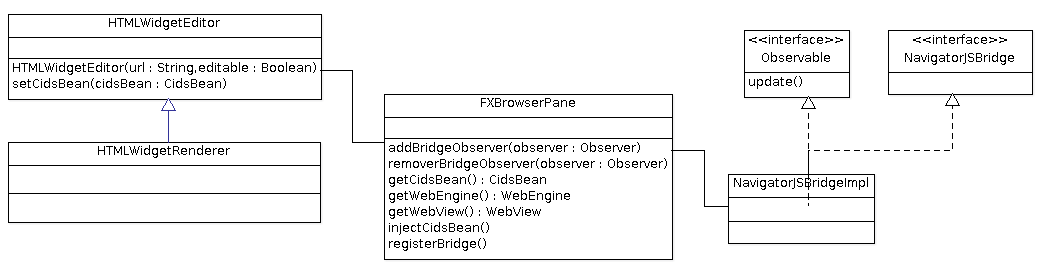
\includegraphics[width=1.0\textwidth]{./img/classDiagramms/html_editor.png}
	\caption{HTMLWidgetEditor and related classes}
	\label{fig:class_diag_html_widget_editor}
\end{figure}


\begin{figure}
	\centering	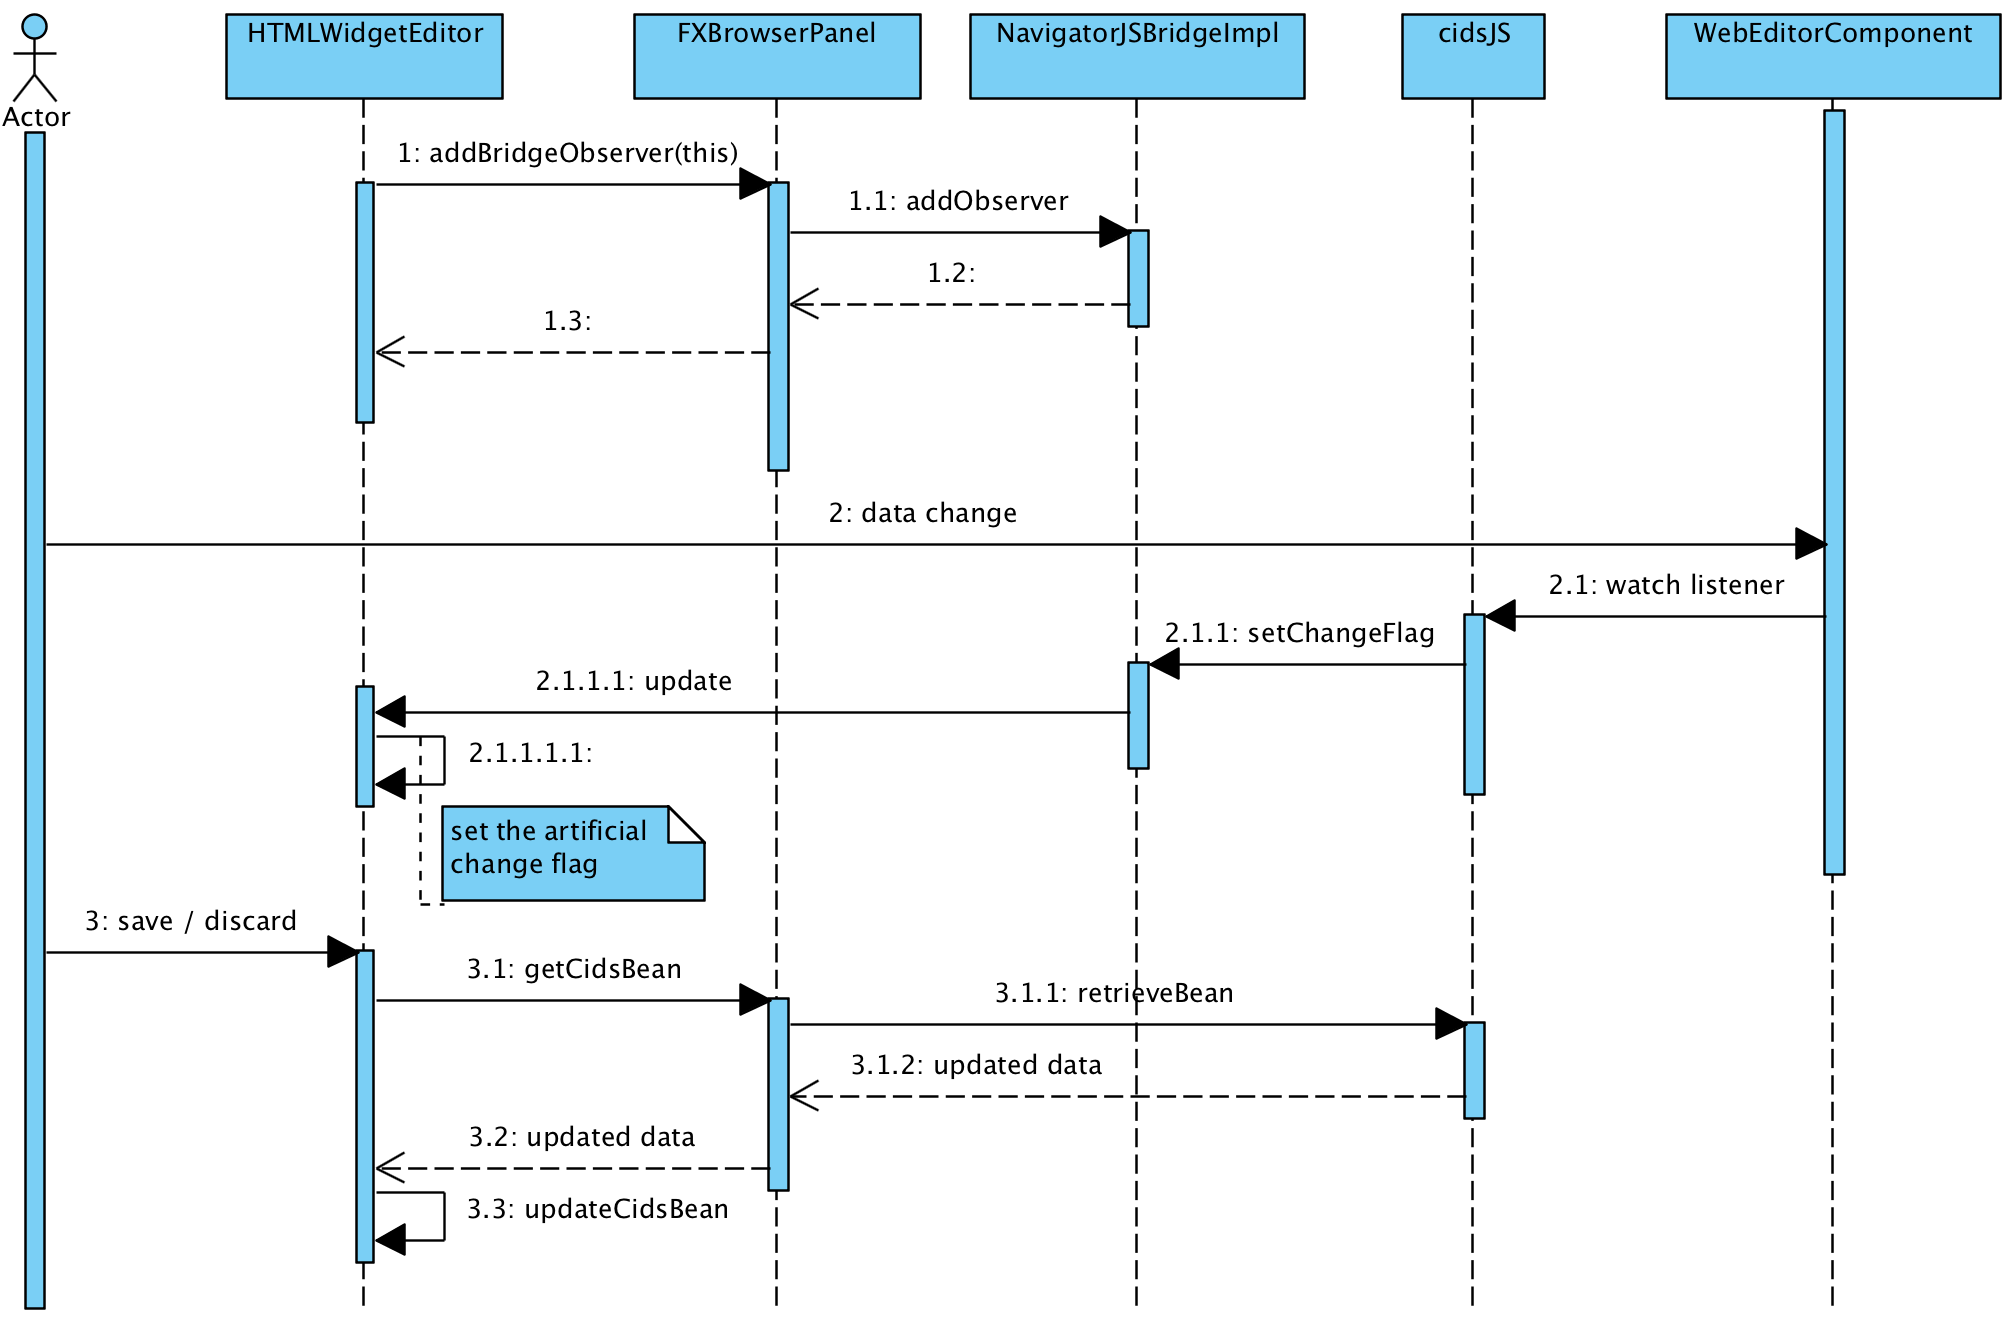
\includegraphics[width=1.0\textwidth]{./img/classDiagramms/seq_diag_data_exchange_2.png}
	\caption{Retrieved CidsBean data from the web editor component}
	\label{fig:seq-diag-data-exchange-2}
\end{figure}

Testing the above described implementation shows that the numerous watches for every property on the \texttt{Cidsbean} slow down the performance of the web editor component.
The reason for this lies in the architecture of Angular.
The watch expressions are checked every time a property on the corresponding scope has changed.
Hence the demo application mainly consists of one scope, all watch expressions are checked every time Angular checks the scope for changes.
Portioning the application into multiple scopes would also solve the problem, but is in conflict with the implemented abstraction of the web application and the backend used.
Hence the main reason of the watches isnjust to indicate that the data has changed, the watches are only needed until the first change in the data has happened. 
After that point the listener mechanism is no longer needed. 
Calling the \texttt{\$watch} function returns a de-registration function that disables the listener mechanism for that watch.
To solve the above mentioned problem, the de-register functions are saved in an array when the watches are set up. The callback function of the watches uses the bridge object to mark the \texttt{CidsBean} as changed. Afterwards, all de-register functions to disable watch-expressions on are executed. 

Hence the data changes are no longer submitted to the \texttt{HTMLWidgetEditor} the artificial change flag of the \texttt{CidsBean} is set when the data has changed. 
Furthermore it is necessary to retrieve the data from the web editor component in case the user wants to save the changes. 
The navigator already provides an interface \texttt{EditorSaveListener} that offers an editor the chance to execute some code before the data is persisted. 
By implementing this interface in the \texttt{HTMLWidgetEditor}, it is possible to retrieve the latest state of the \texttt{CidsBean} with the changes that were made. 
Hence the \texttt{NavigatorAttributeEditorGUI} uses its own reference of the \texttt{CidsBean} it is not possible to assign a new object to the \texttt{CidsBean} field of the \texttt{HtmlWidgetEditor} hence the reference of the \texttt{NavigatorAttributeEditorGUI} points still to the old \texttt{CidsBean} reference. 
Because it is not clear what properties of the \texttt{CidsBean} have changed, the \texttt{CidsBean} class is extended with a method \texttt{bulkUpdate(CidsBean otherBean)} that updates the properties of a \texttt{CidsBean} according to an other instance of a \texttt{CidsBean}. 

Figure \ref{fig:nav_web_editor} depicts the usage of the demo application as editor with the final state of the implemented bi-directional data exchange.

\begin{figure}
	\centering	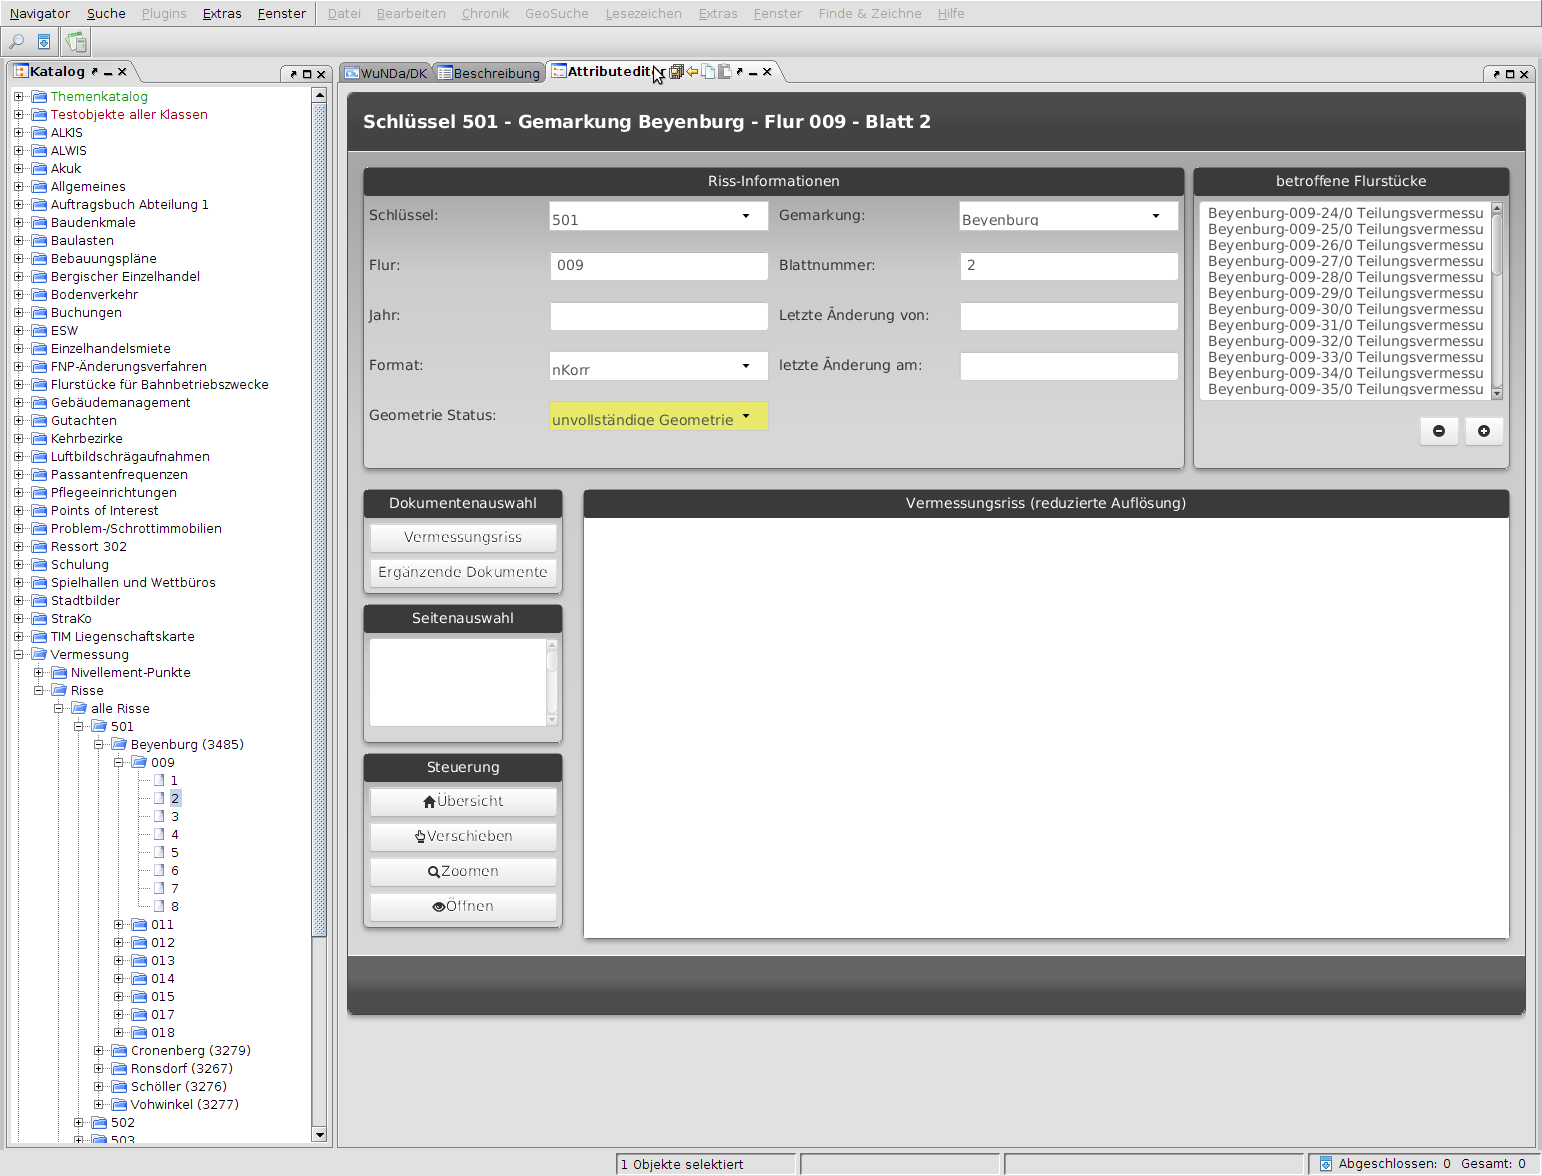
\includegraphics[width=1.0\textwidth]{./img/impl/navigator_web_editor.png}
	\caption{Navigator with Survey Plan Web Editor}
	\label{fig:nav_web_editor}
\end{figure}


\section{Problems and Enhancements}

\subsection{Style of options list}

With the implemented bi-directional data exchange first impressions using the developed survey plan demo application as renderer and editor can be gathered and show some minor problems that still can be improved.

The first issue is, that the option lists of select elements ignore custom css styles. Figure \ref{fig:context_menu} depicts the options list of an select element in the JavaFX WebView. Although the implemenation of the options list is always browser dependent and therefore are only poorly customizable, the most modern browsers allow basic styling of option lists like setting the background color and so on. Unfortuneately the JavaFX WebView uses a JavaFX \texttt{ContextMenu} for implementing the options list of a select element and ignores CSS styles defined in the web application context. 

One central approach of JavaFX is to use a custom implementation of cascading style sheets to separate the layout and content. This implementation is very similar to the CSS implementation used in HTML and relies on the W3C CSS standard 2.1. In \autocite{impl:skinning-fx} a good introduction on styling JavaFX applications is given. A possible solution for solving the above mentioned problem, is to use JavaFX style sheets to adopt the look of the \texttt{ContextMenu} class to better fit into the demo application. Following this approach does not solve the general problem but will provide a sufficient work around. As described in \autocite{impl:skinning-fx}, the JavaFX style sheets are applied to a \texttt{Scene} object. To add styles to a \texttt{Scene} object it is sufficient to provide it with the path of the file that contains the style sheet definitions. The style itself needs to be defined for the class \texttt{.context-menu}. Figure \ref{fig:context_menu_comp}\subref{fig:context_menu_css} shows the options list with the custom CSS.

\begin{figure}
        \centering
        \begin{subfigure}[b]{0.3\textwidth}
                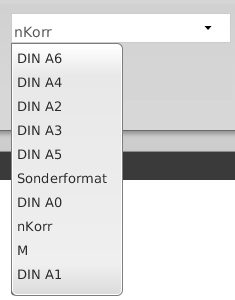
\includegraphics[width=\textwidth]{./img/impl/context_menu.png}
                \caption{Normal State}
                \label{fig:context_menu}
        \end{subfigure}%
        ~ %add desired spacing between images, e. g. ~, \quad, \qquad etc.
          %(or a blank line to force the subfigure onto a new line)
        \begin{subfigure}[b]{0.3\textwidth}
                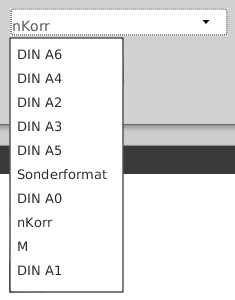
\includegraphics[width=\textwidth]{./img/impl/context_menu_css.png}
                \caption{Custom CSS}
                \label{fig:context_menu_css}
        \end{subfigure}
        ~ %add desired spacing between images, e. g. ~, \quad, \qquad etc.
          %(or a blank line to force the subfigure onto a new line)
        \begin{subfigure}[b]{0.3\textwidth}
                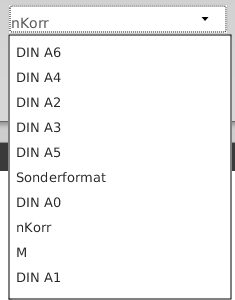
\includegraphics[width=\textwidth]{./img/impl/context_menu_final.png}
                \caption{Skin and CSS}
                \label{fig:context_menu_final}
        \end{subfigure}
        \caption{Design of options list for select elements}\label{fig:context_menu_comp}
\end{figure}

Although the look of the options list now fits more into the look of the demo application there is still the problem that the width of the options list is just as width as the largest element.
A more appropriate visualisation is to extend the width to at least the width of the select element. 
The first idea to use the CSS width property pointed out, that the JavaFX style sheet implementation does not support the width property since layouting in JavaFX is implemented with layout manager objects similar to Swing. 
A possible workaround is to provide a custom skin class for context menus, that is used when a \texttt{ContextMenu} object is generated. 
A good explanation for this procedure can be found in \autocite{impl:fx-ui-controls}. 
To put it in a nutshell, every JavaFX component is composed by a control, a skin and a behaviour class. 
This approach is very similar to Java Swing where very component also has an UI class that combines the tasks of skin, control and behaviour. 
Figure \ref{fig:fx-skinning} demonstrates this.

\begin{figure}
	\centering 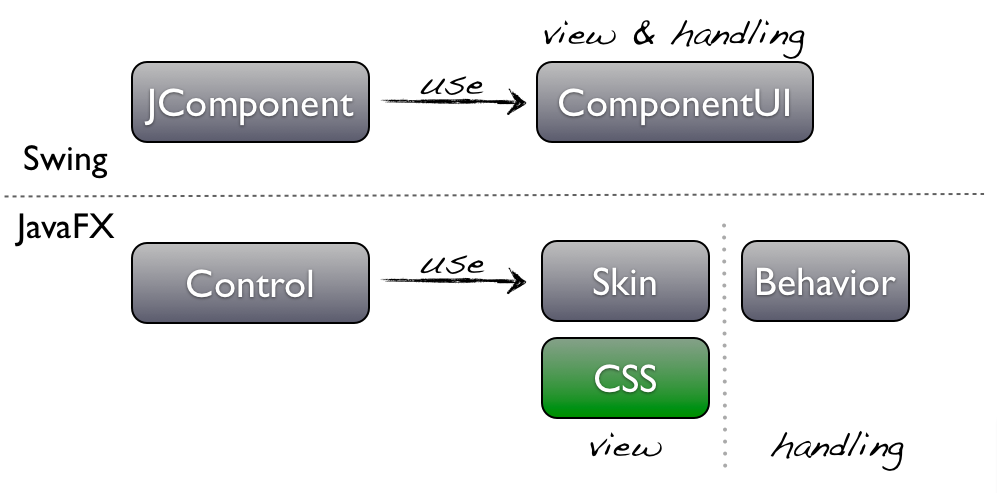
\includegraphics[width=1.0\textwidth]{./img/impl/fx_components.png}
	\caption{Architecture of javaFX Components in contrast to Java Swing, \autocite{impl:fx-ui-controls}}
	\label{fig:fx-skinning}
\end{figure}

In the constructor of the custom skin class for context menus we wrap the existing menu items into an rectangle that has the same width of the select element and replace the menu items of the context menu. 
Figure \ref{fig:context_menu_final} shows the final state of the options list for select elements.

\subsection{ Avoiding flickr effect during load}

Another problem that can be regarded is that the web application is already visualised although it is not finally initialised.
The user can observe a flickering effect of multiple different states, each one only present for a short time. 
Normally the description pane and the editor panel show a waiting symbol until the final renderer or swing component is initialized. 
In the case of web applications there are two more different states depicted in figure \ref{fig:flickering}.

\begin{figure}
\centering 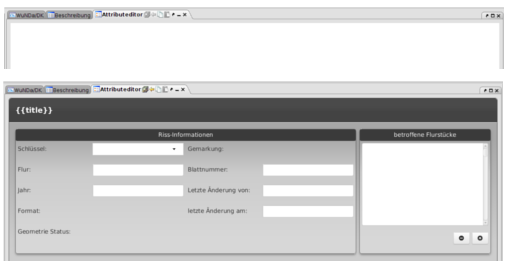
\includegraphics[width=1.0\textwidth]{./img/impl/flickering_states.png}
	\caption{Flickering states}
	\label{fig:flickering}
\end{figure}
The first state is a totally white panel. This white panel represents the JavaFX WebView container. Hence the web page is not totally loaded at this point, the WebView just renders a simple white background. 
In the second state, the web page is completely loaded because the HTML and CSS parts of the application are already visible. 
But instead of the actual data, the user can see the binding expressions that are used in the HTML mark-up to enable the data binding in Angular. 
This is a very common problem in angular and is documented in \autocite{impl:ng-cloak}, \autocite{impl:ng-bind} and \autocite{impl:stackoverflow-ng-cloak}. 
The problem is, that the templates are already visualised before they are compiled from Angular, or in other words, the web page is totally loaded, however the Angular application is not totally initialized. 
The Angular documentation offers two possibilities to work around this issue, the first one is to use a special directive \texttt{ng-cloak}. 
The Angular documentation states that the \texttt{ng-cloak} directive can be used to \enquote{[...] prevent the Angular html template from being briefly displayed by the browser in its raw (uncompiled) form while your application is loading. Use this directive to avoid the undesirable flicker effect caused by the html template display.} \autocite{impl:ng-cloak}
Unfortunately using this directive didn't work for a unknown reason. 
The second solution is to use the \texttt{ng-bind} directive instead of the double curly braces notation.
Using the \texttt{ng-bind} directive hides the curly braces, however, the user still has a flickering effect when the templates are compiled and the data is inserted.

To totally avoid those flickering effects another solution is needed. 
The main reason why those multiple states are visible to the user, is that the navigator assumes that the renderer respective the editor is completely initialized after the \texttt{setCidsBean} method is called. 
Despite this is true for Swing based renderer, this is not true for the \texttt{HtmlWidgetEditor}, hence the web page is asynchronously loaded. 
Thus, the renderer and editor loading mechanism needs to be blocked until the web application is completely initialized. 

The first problem to solve when trying to implement the above outlined work around, is to determine when the angular application has finished the intitialisation of the application. 
In fact Angular does not fire a event for that case, it is necessary to understand how an angular application is bootstrapped. 
The chain of actions that happen during the initialisation are described in \autocite{impl:ng-bootstrap} but without going into great detail one of the latest things is setting up the controllers. 
In fact we have delayed the initialisation of the application to the point all relevant data is available the \texttt{SurveyPlanController} function is executed and after the Angular application is initialised. We can easily extend the \texttt{SurveyPlanController} to send a signal back to the navigator. 
In order to do so, the cidsJS layer and the interface of the bridge object are extended with corresponding methods.

Now that web editor component application notifies the bridge object as soon as it is initialised the loading process needs to be delayed up to this point. 
For this a new interface, named \texttt{InitialisationLocker}, is introduced that basically has a method that returns a \texttt{CountDownLatch} object. 
A \texttt{CountDownLatch} allows one or more threads to wait until a other thread completes its execution. 
It is initialized with a given value. Additionally the await method of the \texttt{CountDownLatch} will block until the value oof it reaches zero. 
The thread in that the \texttt{DescriptionPane} loads the renderer needs to check if the renderer that is currently loaded implements the \texttt{InitialisationLocker} interface and calls the await method of the \texttt{CountDownLatch} this interface provides.
This causes to block the thread of the loading mechanism. 
If the web application sends the message that it is initialised, the \texttt{HtmlWidgetEditor} counts down the value of the \texttt{CountDownLatch} which reverses the blocked status renderer loading thread. 

Testing the above mentioned changes shows an unexpected result. 
At the very beginning there is still a stutter with a white area until the web application is displayed. 
Further investigation on that issue shows that the JavaFX WebView starts its rendering process just in the case the WebView is visible. 
In \autocite{impl:fx-snapshot} a possible solution is described. 
The idea is to do a snapshot of the WebView in the background. 
This initiates the internal rendering process. 
